\chapter{Project Management and Development Evidence}

This chapter records implementation, repository, testing, tool-use, and risk evidence available for the current SABLE branch. Team-wide claims are limited to evidence visible in the shared repository. Contributions for other modules should be reconciled against their own branches and commits before the complete team report is submitted.

\section{Work Completed}

The current SABLE contribution includes a local Terraform/HCL analysis pipeline, a bounded IAM/S3 authorization evaluator, successor correspondence, explicit outcomes of \texttt{PRESERVED}, \texttt{REGRESSED}, and \texttt{UNKNOWN}, baseline comparisons B0--B4, authored scenarios, and integration with the shared evidence/final-gate path. Automated tests cover expected results, unsupported and ambiguous inputs, stale evidence, input-hash mismatch, and evidence integrity. The unresolved-role-binding correction is commit \texttt{58b0a3d}; it is included in verified combined commit \texttt{665b224} on \texttt{integration/sable-satra-cavr}. The 27-pass local audit and 44-pass initial CI results are historical, separate results; the focused shared-assurance CI on the combined snapshot passed 46 tests.

The initial SABLE changes were published on the team's \texttt{sable} branch. The current verification point is the isolated combined branch \texttt{integration/sable-satra-cavr} at \texttt{665b224}; it contains the integrated CAVR, SATRA-RV, SABLE, and shared workflow snapshot. It is not merged into \texttt{master}. The SABLE shared-assurance job on this commit passed 46 tests.

\subsection{Rendered Application Evidence}
The integrated capture below comes from the shared ASENT Run Workflow, not from the dedicated SABLE page. It records run \texttt{104074afe883} for the \texttt{sable\_regressed} storage-refactor scenario. The displayed module outcomes are CAVR \texttt{VERIFIED}, SABLE \texttt{REGRESSED}, and SATRA \texttt{INCONCLUSIVE}, with an overall final decision of \texttt{BLOCK}. The trace shows a known obligation that does not hold and a candidate policy target changed through the storage module. Since SATRA is also inconclusive, the screenshot is not evidence that SABLE was the sole cause of the overall gate result.

\begin{figure}[p]
    \centering
    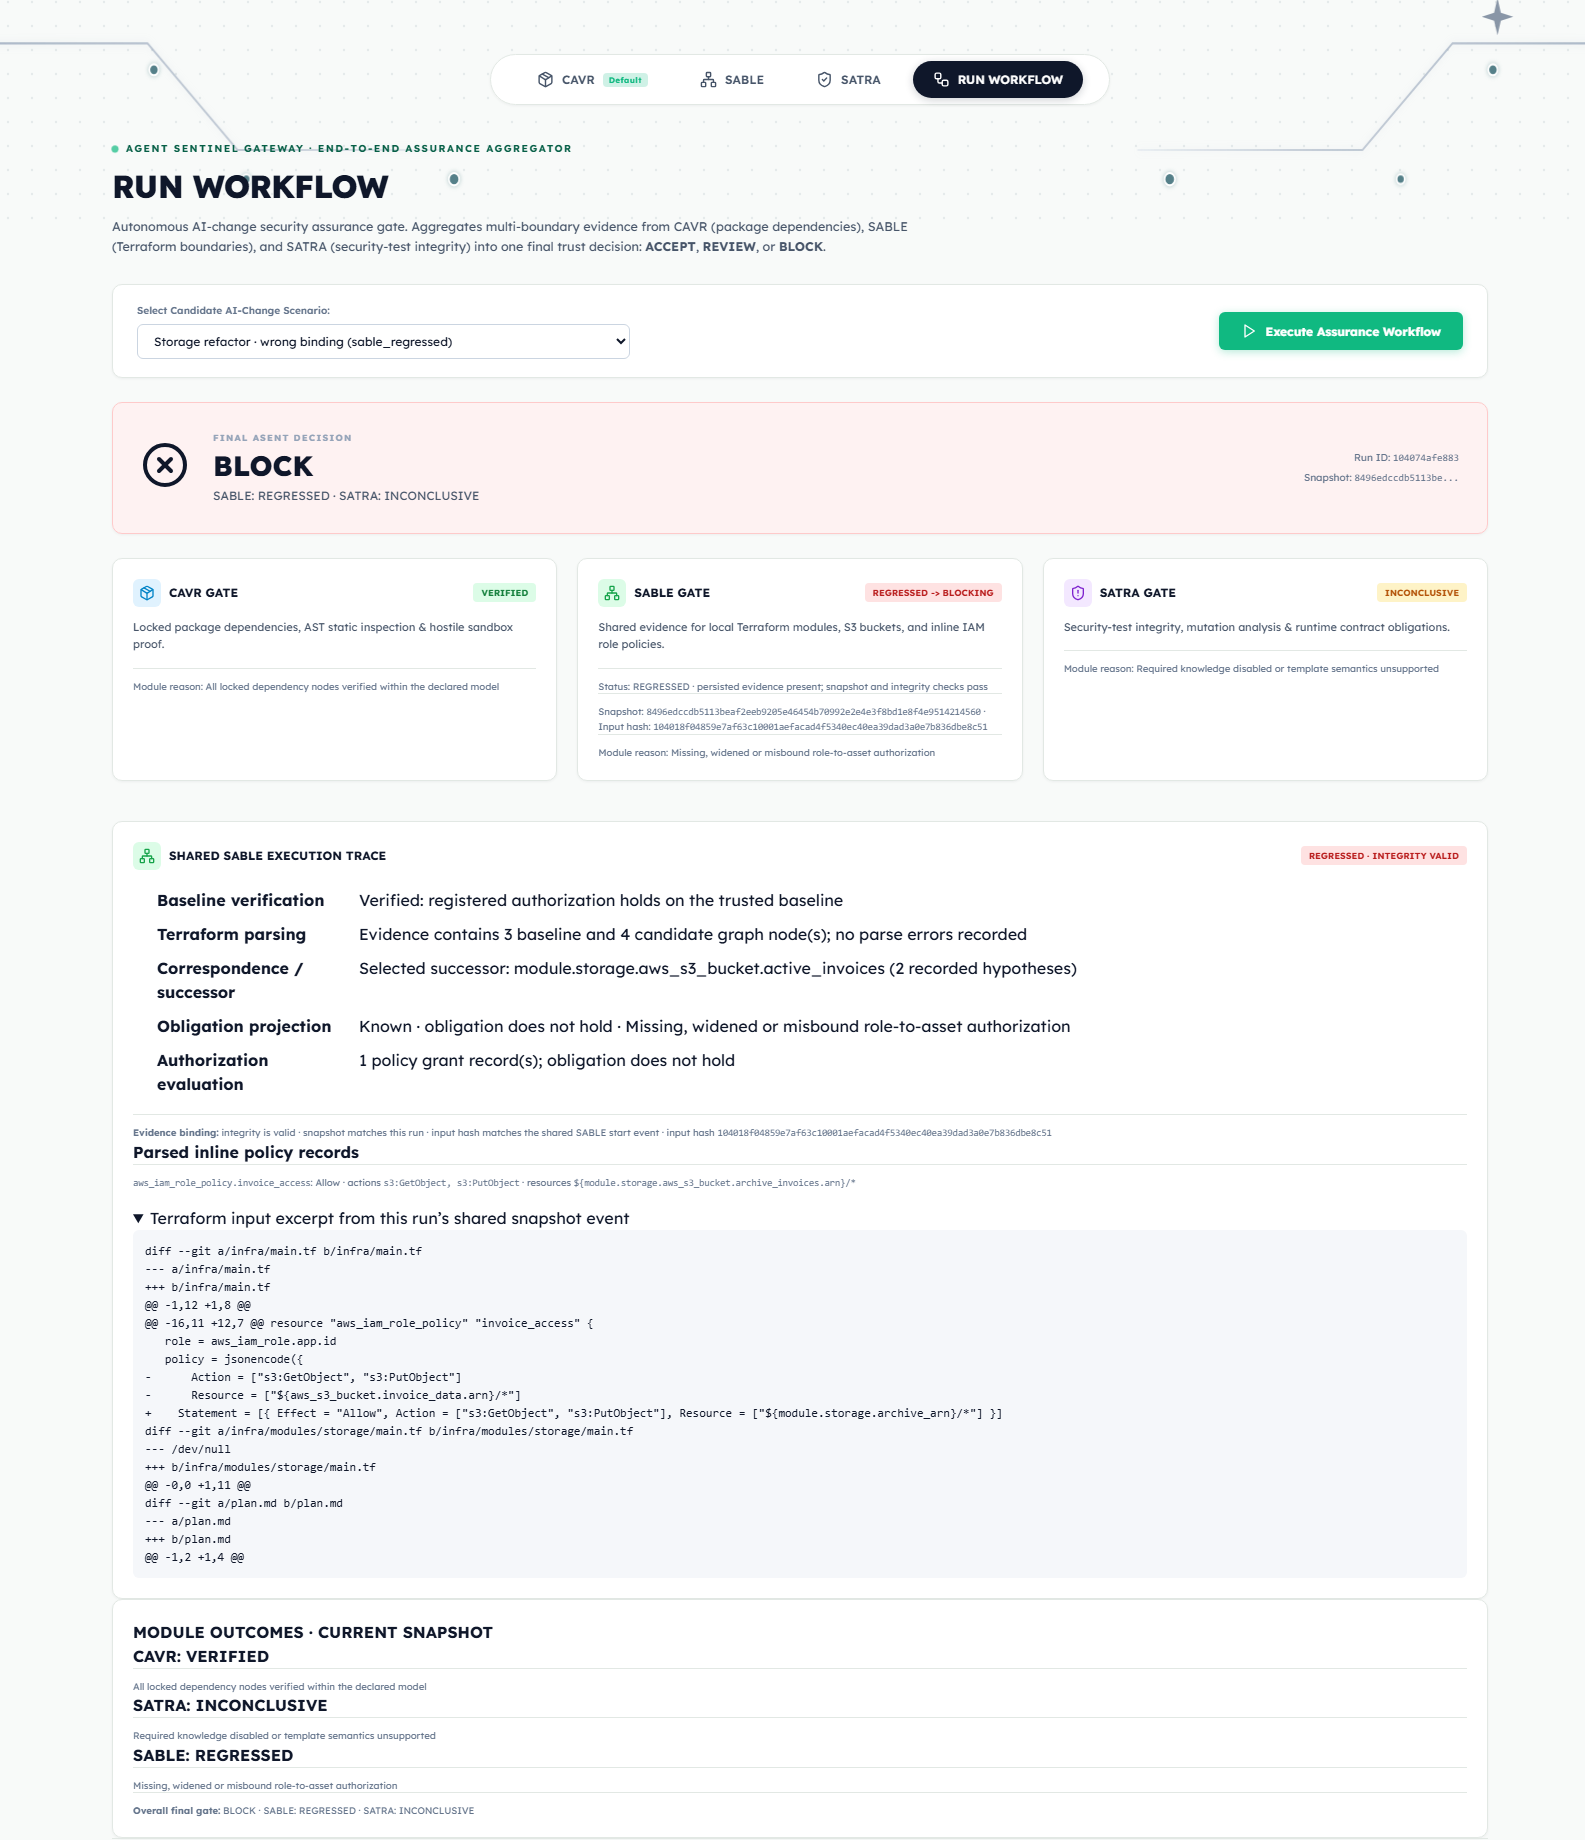
\includegraphics[width=0.98\textwidth,height=0.79\textheight,keepaspectratio]{ThesisFigs/asent_shared_sable_regressed_workflow_detail.png}
    \caption{Integrated ASENT Run Workflow for run \texttt{104074afe883}: shared SABLE evidence, candidate Terraform excerpt, module results, and final-gate decision.}
    \label{fig:asent-shared-sable-regressed}
\end{figure}
\clearpage

A separate capture from the dedicated SABLE page covers the distinct \texttt{policy\_\allowbreak{}rewrite\_\allowbreak{}wrong\_\allowbreak{}target} case and the \texttt{S3-\allowbreak{}APPROLE-\allowbreak{}CUSTOMERDATA} obligation. It is a different scenario from the integrated invoice-storage run above.

\begin{figure}[!htbp]
    \centering
    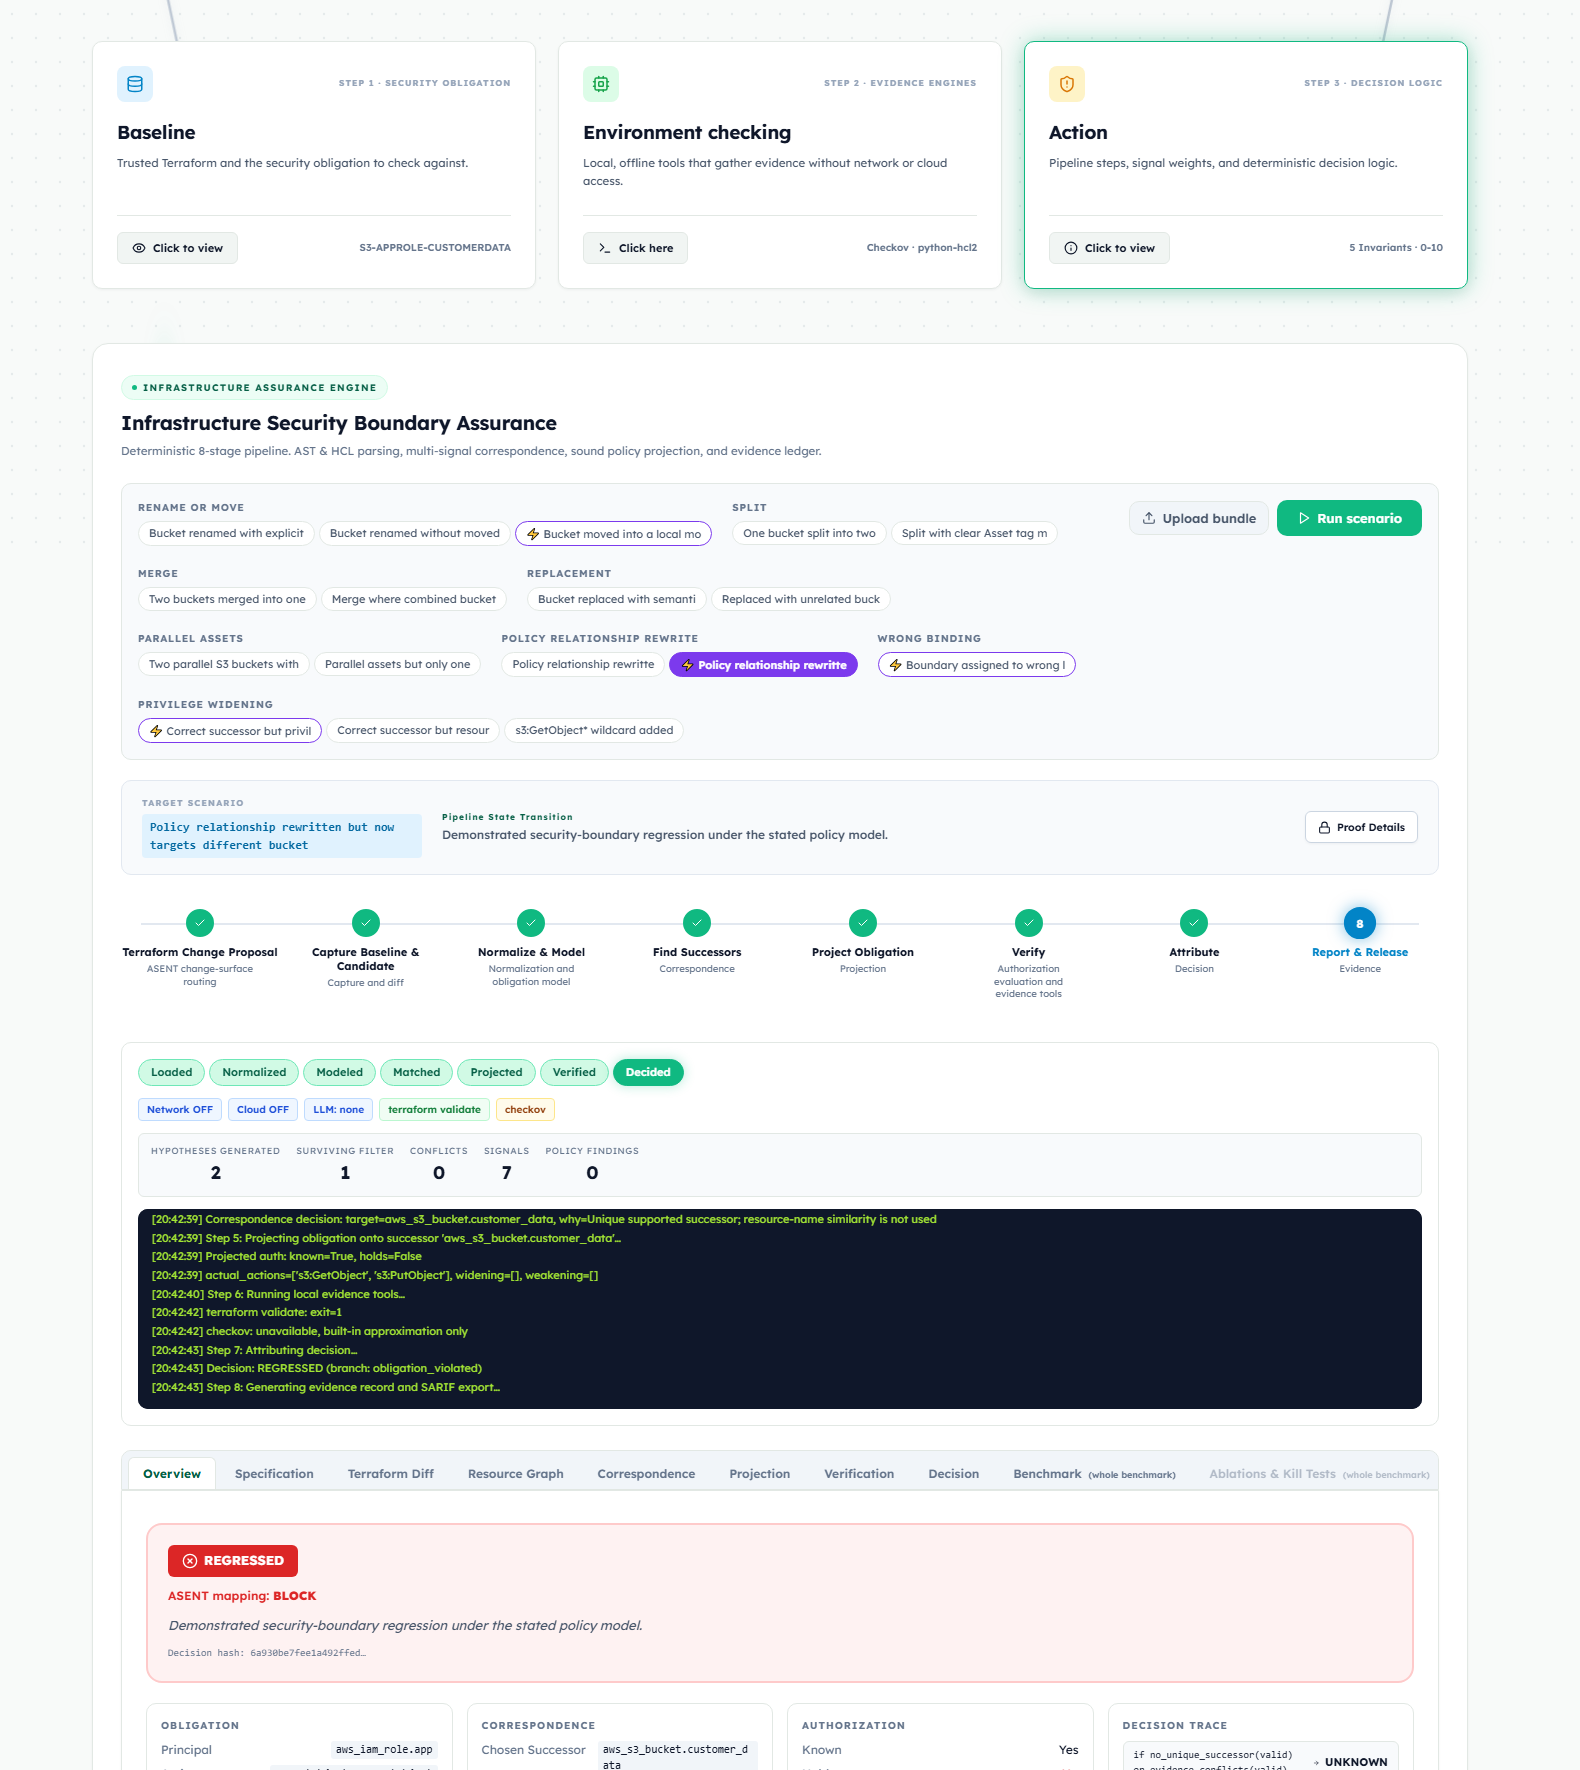
\includegraphics[width=0.96\textwidth,height=0.73\textheight,keepaspectratio]{ThesisFigs/sable_wrong_target_result_detail_crop.png}
    \caption{Dedicated SABLE page: wrong-target scenario result for the \texttt{S3-APPROLE-CUSTOMERDATA} obligation. The UI reports \texttt{REGRESSED}, mapped to \texttt{BLOCK}.}
    \label{fig:sable-customer-data-result}
\end{figure}
\clearpage

\begin{figure}[htbp]
    \centering
    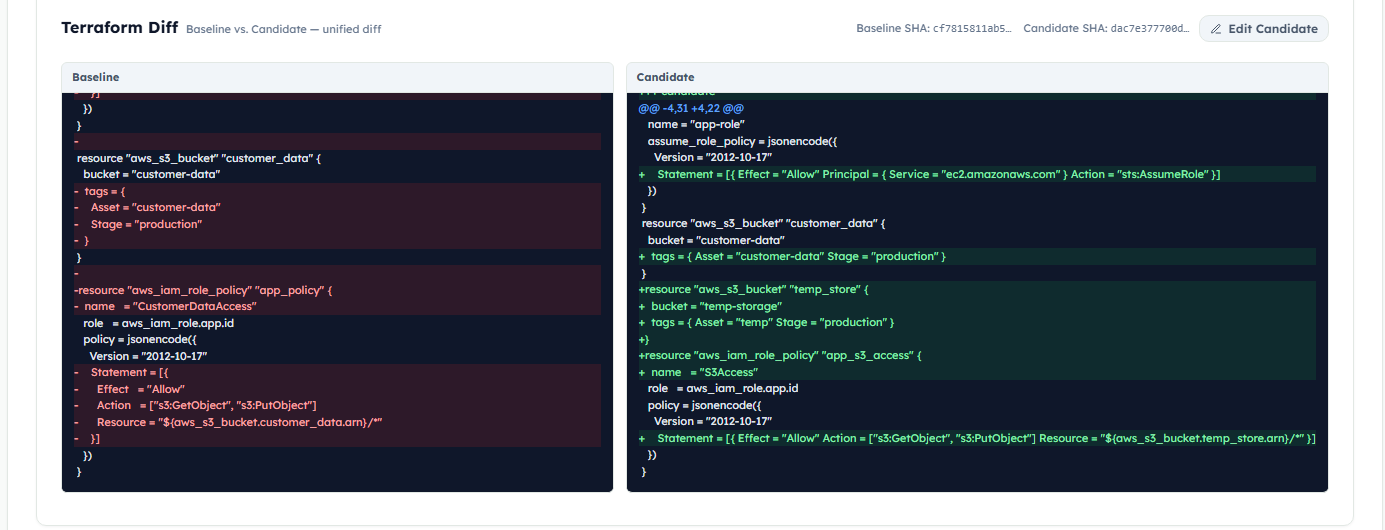
\includegraphics[width=0.99\textwidth,height=0.32\textheight,keepaspectratio]{ThesisFigs/sable_wrong_target_policy_comparison_crop.png}
    \caption{Dedicated SABLE wrong-target scenario: baseline authorization points to the \texttt{customer\_data} bucket, while the candidate policy targets \texttt{temp\_storage}.}
    \label{fig:sable-customer-data-policy-diff}
\end{figure}

The two dedicated-page report figures are focused crops of the saved UI captures; only the visible area was trimmed for readability and the displayed application content was not changed. They support the distinct \texttt{policy\_rewrite\_wrong\_target} scenario, associated with local run \texttt{sable-1791646956750}: the \texttt{S3-APPROLE-CUSTOMERDATA} obligation and policy target change from \texttt{customer\_data} to \texttt{temp\_storage}. These are not screenshots of the integrated invoice-storage run above. None of the screenshots establishes live AWS behavior or applied infrastructure.

\subsection{Earlier Shared-Workflow Rehearsal}
At branch head \texttt{753a55b} on \texttt{sable}, the shared Run Workflow was executed for three mid-evaluation outcomes. These earlier aggregate runs are kept separate from the latest dedicated SABLE module screenshots below. The run records completed with the following module and aggregate decisions:

\small
\setlength{\tabcolsep}{2pt}
\begin{longtable}{p{0.14\textwidth}p{0.15\textwidth}p{0.14\textwidth}p{0.27\textwidth}p{0.16\textwidth}}
\toprule
\textbf{Scenario} & \textbf{Run ID} & \textbf{SABLE} & \textbf{Final gate} & \textbf{Evidence binding}\\
\midrule
\endhead
\path{sable_preserved} & \texttt{b107fd\allowbreak{}8f0f2f} & \texttt{PRESERVED} & \texttt{REVIEW}; SATRA \texttt{INCONCLUSIVE} & Integrity valid; snapshot and input hash match\\
\path{sable_regressed} & \texttt{5c6fe1\allowbreak{}aa3a96} & \texttt{REGRESSED} & \texttt{BLOCK}; SABLE \texttt{REGRESSED}; SATRA \texttt{INCONCLUSIVE} & Integrity valid; snapshot and input hash match\\
\path{sable_unknown} & \texttt{b6d358\allowbreak{}8ec006} & \texttt{UNKNOWN} & \texttt{REVIEW}; SABLE \texttt{UNKNOWN}; SATRA \texttt{INCONCLUSIVE} & Integrity valid; snapshot and input hash match\\
\bottomrule
\end{longtable}
\normalsize
\setlength{\tabcolsep}{6pt}
The \texttt{PRESERVED} result is not an overall \texttt{ACCEPT}: the shared gate returned \texttt{REVIEW} because SATRA was \texttt{INCONCLUSIVE}. For every row, the SABLE evidence record was integrity-valid, its candidate snapshot matched the run, and its input hash matched the SABLE start event.

\begin{sloppypar}
The current-checkout image for run \texttt{b6d358\allowbreak{}8ec006} is an intermediate UI capture. It visibly shows SABLE \texttt{UNKNOWN} and the \texttt{REVIEW} headline, but the gate explanation still says the candidate is waiting for evidence and the CAVR card has no current evidence. The persisted run subsequently reached \texttt{COMPLETE} with final-gate reasons \texttt{SATRA: INCONCLUSIVE} and \texttt{SABLE: UNKNOWN}. Browser runtime initialization blocked a fresh completed-state screenshot, so this intermediate image is not cited as proof of the final gate explanation. The runbook records the exact image path and limitation.
\end{sloppypar}

\subsection{Latest SABLE Module UI Demonstration}
The following results are from the dedicated SABLE page exercised on the verified combined source snapshot at \texttt{665b224}. The UI displays the registered obligation, the baseline/candidate Terraform evidence, the analysis trace, a SABLE verdict, its SABLE-to-ASENT mapping, and an evidence-chain verification result. The mapping in this table is the SABLE module's displayed outcome; it is not a claim that the complete shared workflow has the same final decision for every run.

\small
\setlength{\tabcolsep}{5pt}
\begin{longtable}{p{0.24\textwidth}p{0.20\textwidth}p{0.18\textwidth}p{0.22\textwidth}}
\toprule
\textbf{Scenario} & \textbf{SABLE verdict} & \textbf{SABLE mapping} & \textbf{Evidence chain}\\
\midrule
\endhead
\path{rename_with_moved} & \texttt{PRESERVED} & \texttt{ACCEPT} & 9 of 9 records verified\\
\path{privilege_widening} & \texttt{REGRESSED} & \texttt{BLOCK} & 9 of 9 records verified\\
\path{split_to_two} & \texttt{UNKNOWN} & \texttt{REVIEW} & 7 of 7 records verified\\
\bottomrule
\end{longtable}
\normalsize
\setlength{\tabcolsep}{6pt}

The preserved case uses an explicit Terraform \texttt{moved} block and retains the registered IAM role's S3 actions and customer-data resource scope. The privilege-widening case adds a wildcard action/resource grant on the identified successor and is classified as a known regression. The split case leaves two plausible successors too close for unique attribution; SABLE abstains with \texttt{UNKNOWN}. The authorization decision path is deterministic and does not rely on an LLM. The checks analyze supplied Terraform and IAM evidence; they do not apply infrastructure to AWS.

\begin{figure}[p]
    \centering
    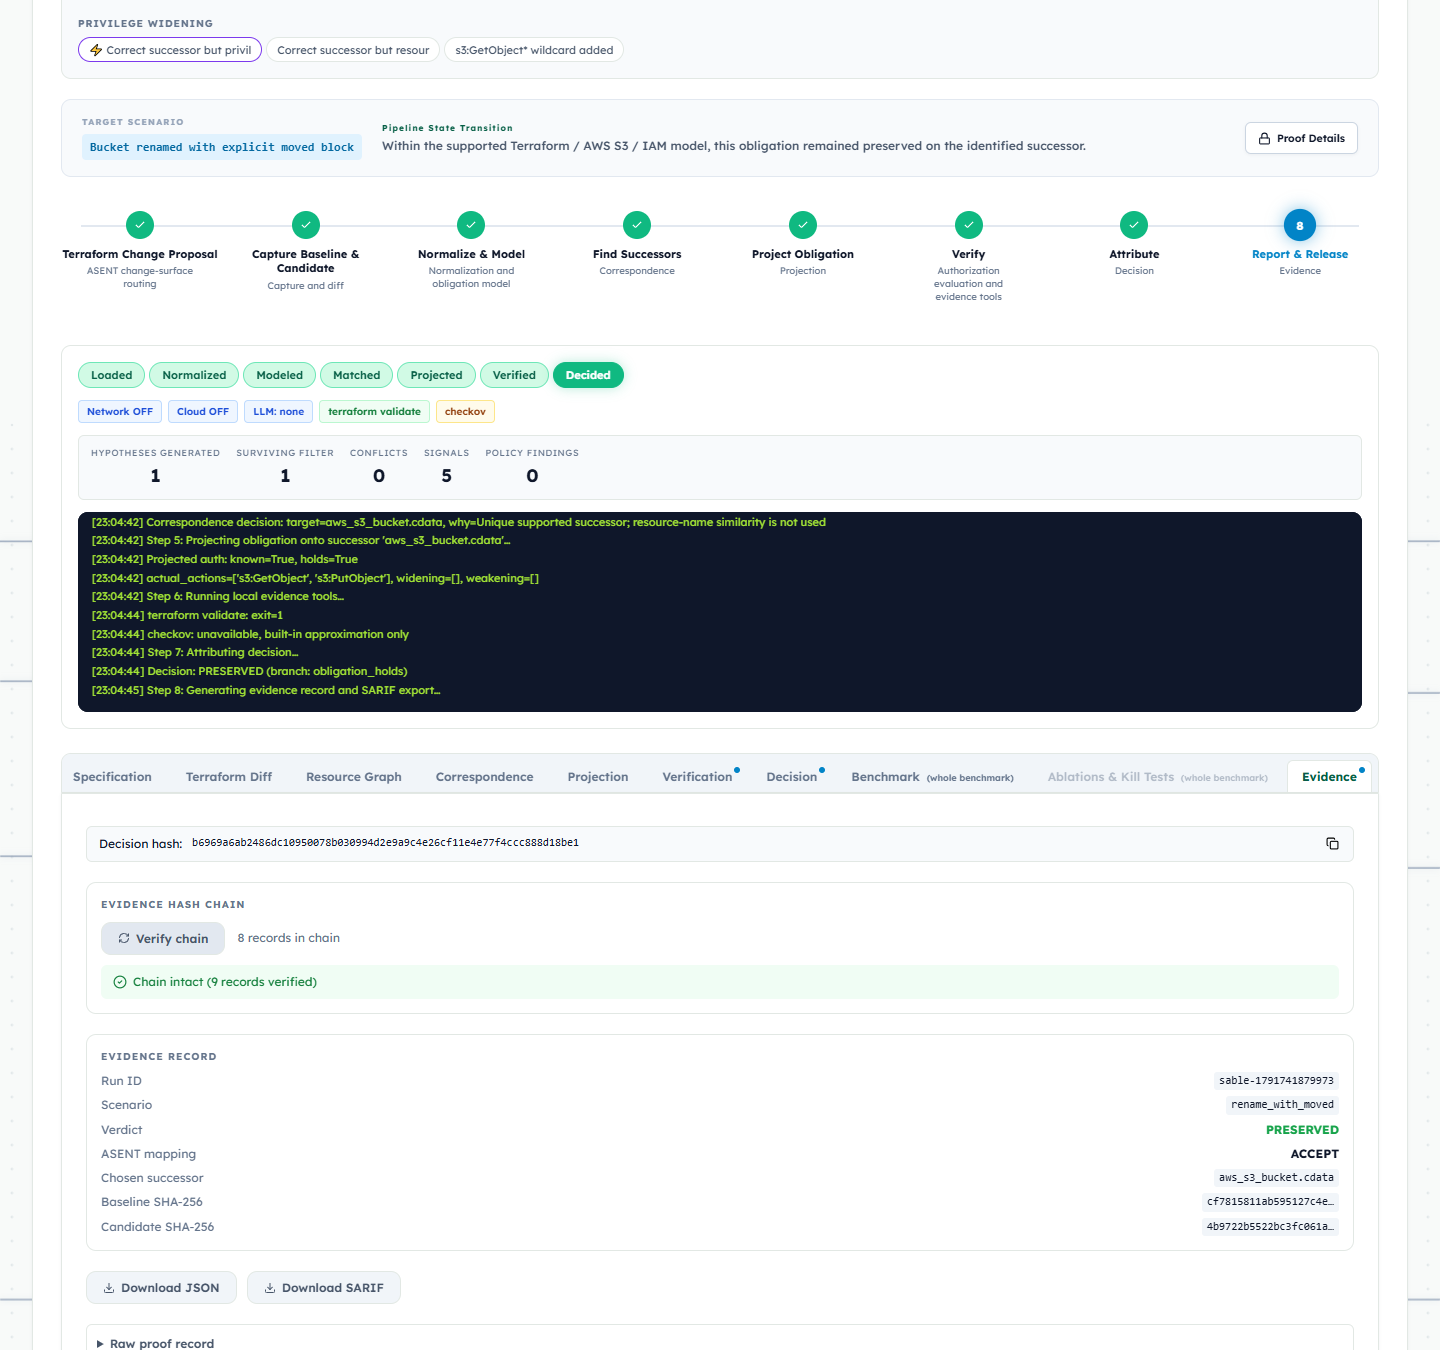
\includegraphics[width=0.98\textwidth,height=0.72\textheight,keepaspectratio]{figures/sable/rename-with-moved-chain-detail.png}
    \caption[SABLE UI: preserved rename with move]{Dedicated SABLE UI evidence for \texttt{rename\_with\_moved}: preserved obligation, SABLE mapping \texttt{ACCEPT}, and an intact chain with nine records verified. Cropped from the original full-page capture for readability.}
    \label{fig:sable-ui-preserved-evidence}
\end{figure}
\clearpage

\begin{figure}[p]
    \centering
    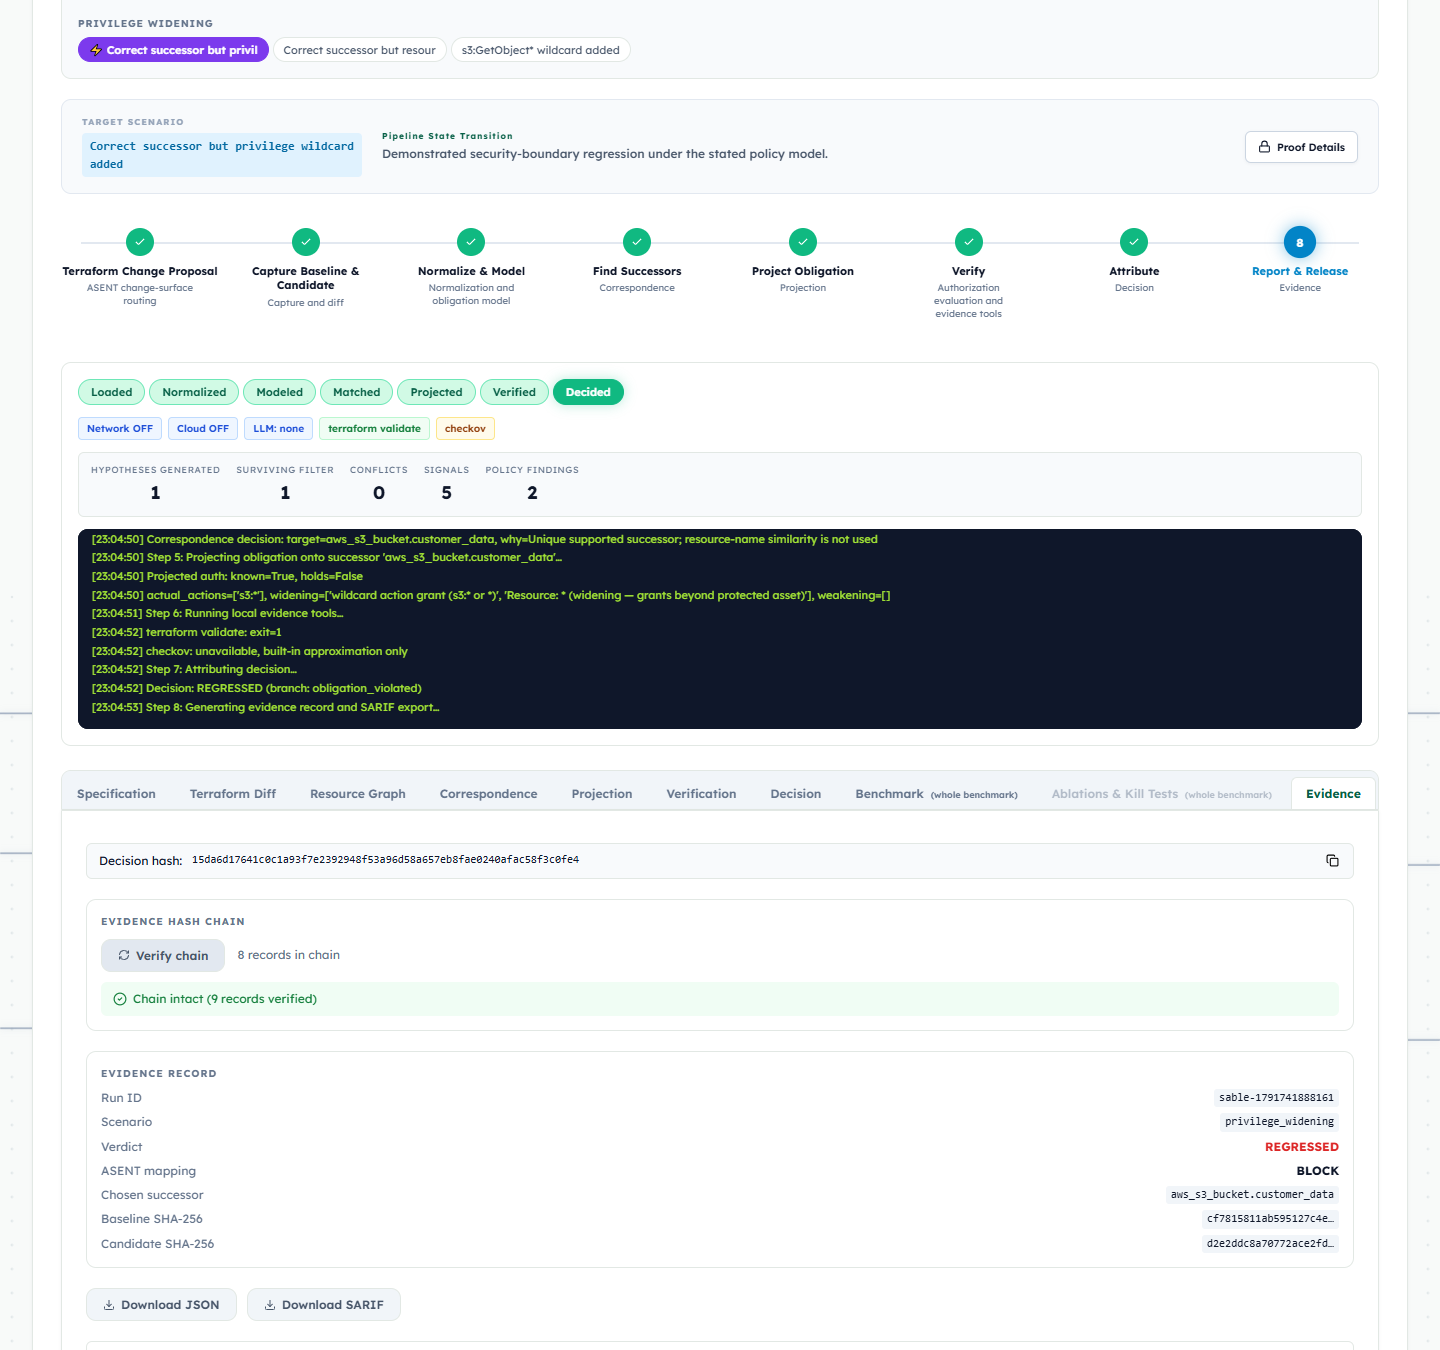
\includegraphics[width=0.98\textwidth,height=0.72\textheight,keepaspectratio]{figures/sable/privilege-widening-chain-detail.png}
    \caption[SABLE UI: privilege widening regression]{Dedicated SABLE UI evidence for \texttt{privilege\_widening}: the widened grant is classified \texttt{REGRESSED}/\texttt{BLOCK}; the evidence chain verifies nine records. Cropped from the original full-page capture for readability.}
    \label{fig:sable-ui-regressed-evidence}
\end{figure}
\clearpage

\begin{figure}[p]
    \centering
    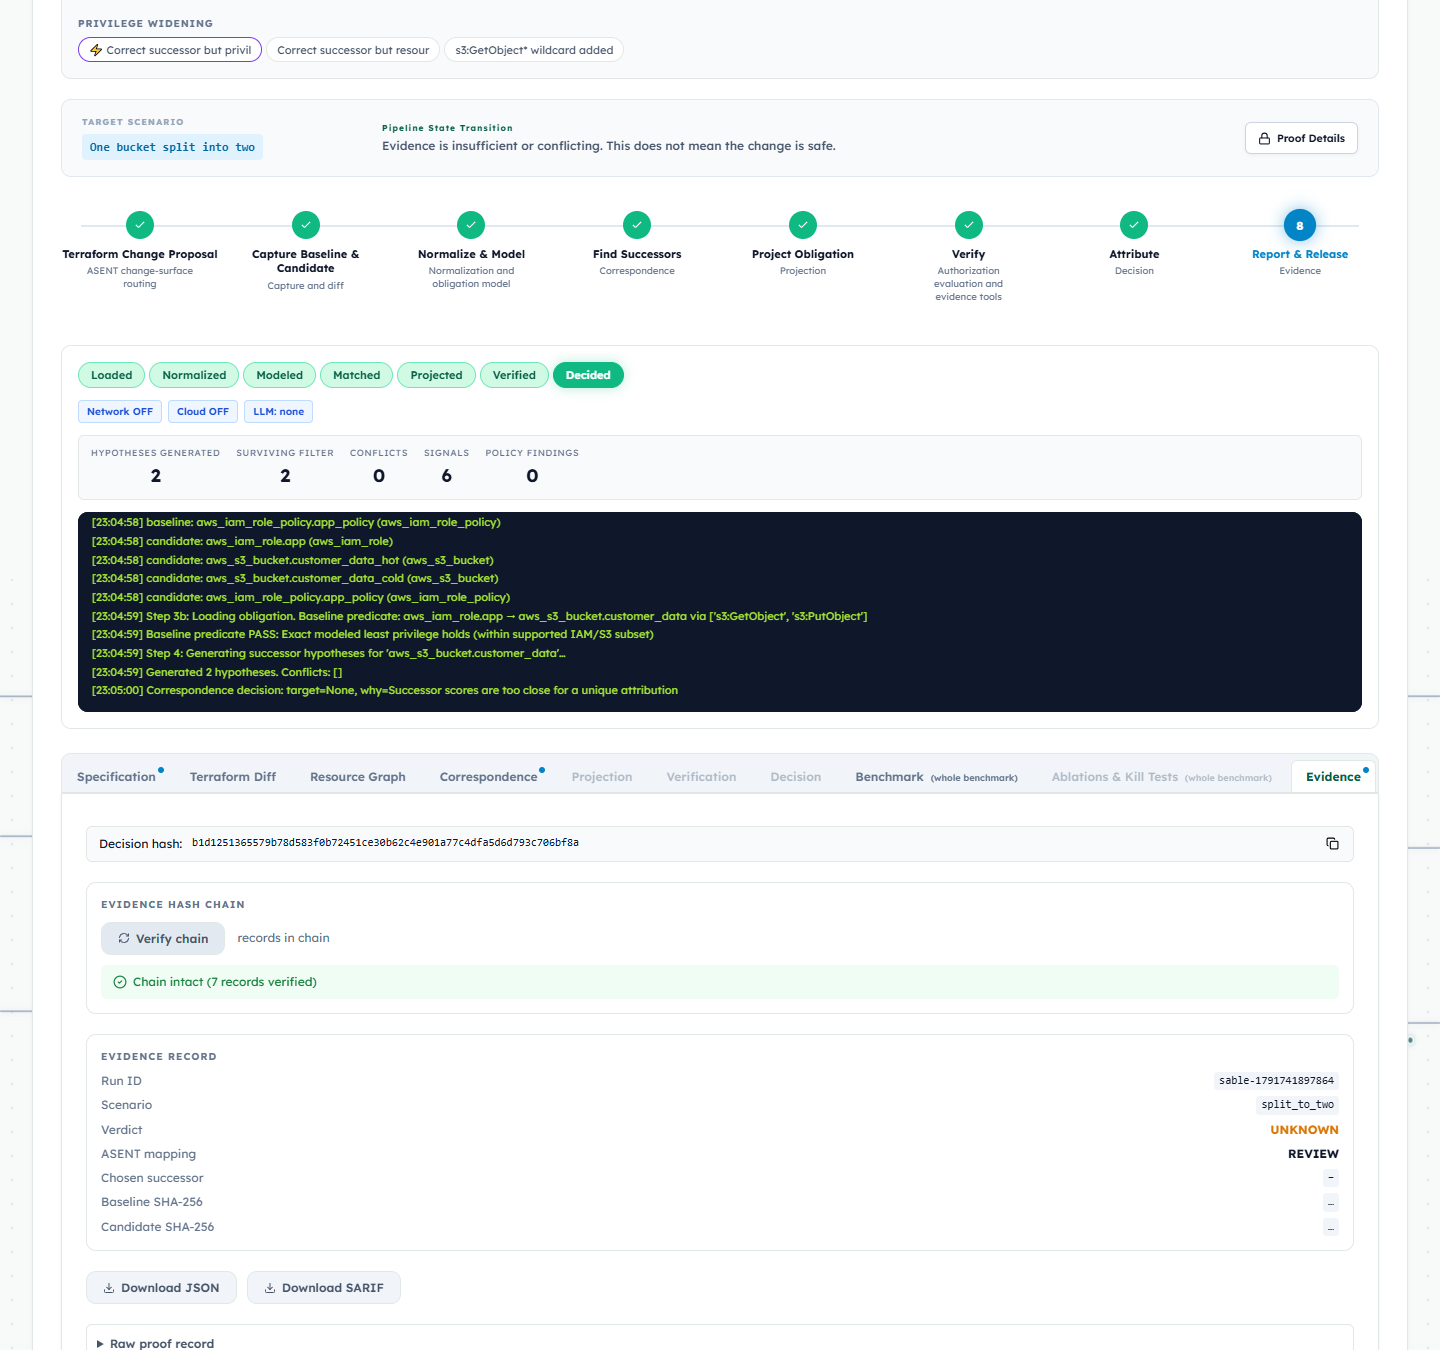
\includegraphics[width=0.98\textwidth,height=0.72\textheight,keepaspectratio]{figures/sable/split-to-two-chain-detail.png}
    \caption[SABLE UI: ambiguous split review]{Dedicated SABLE UI evidence for \texttt{split\_to\_two}: ambiguous correspondence returns \texttt{UNKNOWN}/\texttt{REVIEW}; the evidence chain verifies seven records. Cropped from the original full-page capture for readability.}
    \label{fig:sable-ui-unknown-evidence}
\end{figure}
\clearpage

\begin{figure}[p]
    \centering
    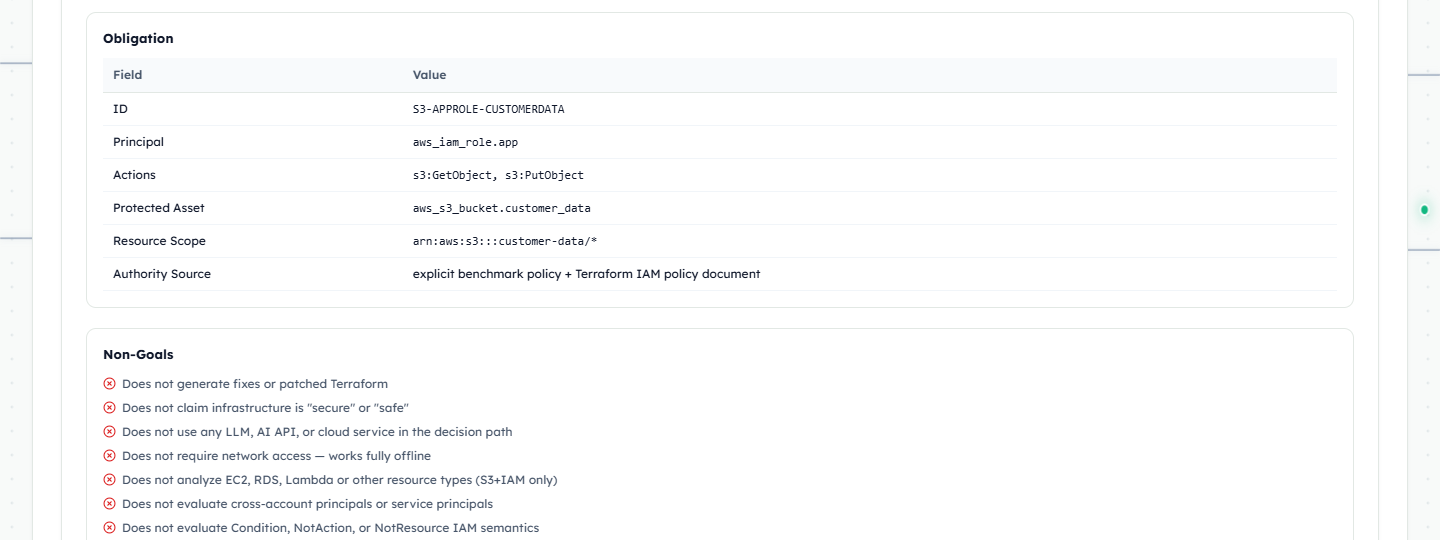
\includegraphics[width=0.96\textwidth,height=0.70\textheight,keepaspectratio]{figures/sable/registered-obligation-detail.png}
    \caption[SABLE UI: registered obligation]{SABLE UI input evidence: the registered \texttt{S3-APPROLE-CUSTOMERDATA} principal, action, and resource scope. This is unaltered UI content cropped to the relevant panel.}
    \label{fig:sable-ui-obligation-and-terraform}
\end{figure}
\clearpage

\begin{figure}[p]
    \centering
    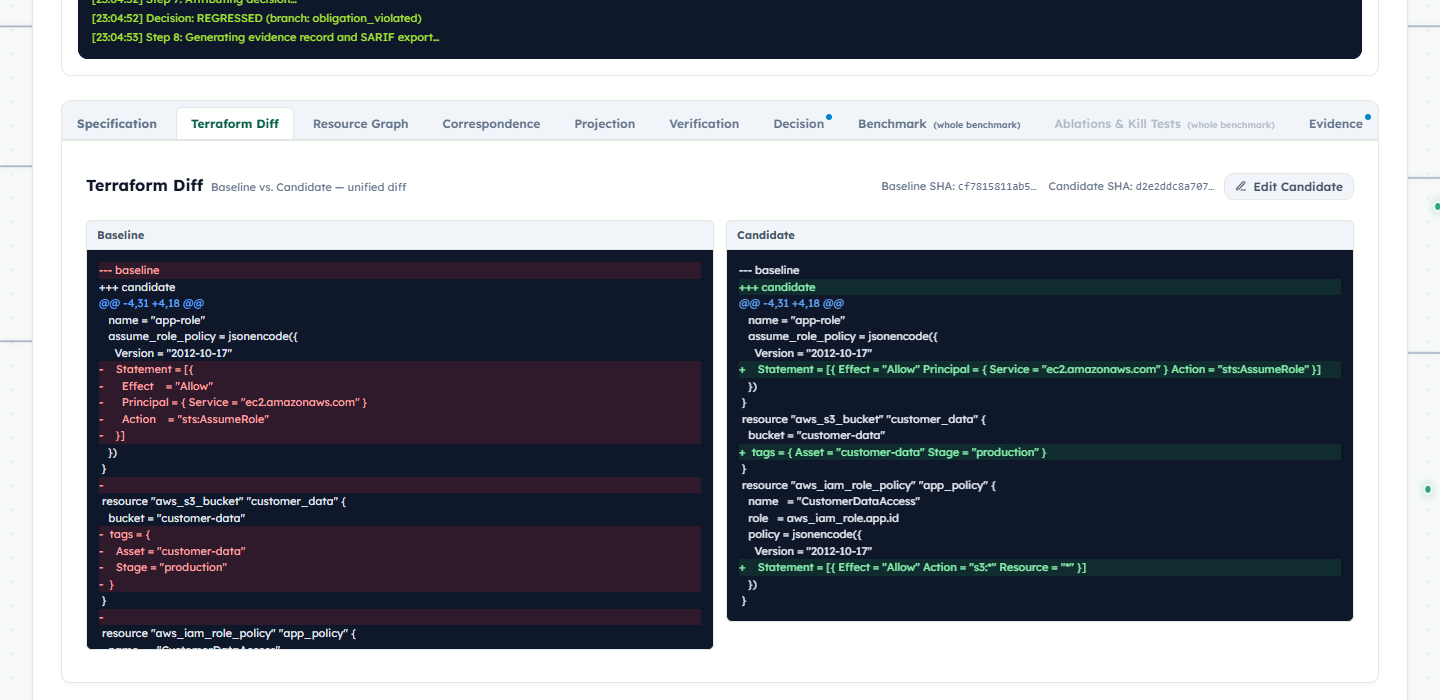
\includegraphics[width=0.96\textwidth,height=0.60\textheight,keepaspectratio]{figures/sable/terraform-diff-detail.png}
    \caption[SABLE UI: Terraform baseline and candidate]{Baseline/candidate Terraform diff shown in the privilege-widening demonstration. The screenshot is cropped to the application panel; the displayed Terraform content is unchanged.}
    \label{fig:sable-ui-terraform-diff}
\end{figure}
\clearpage

\section{Work Remaining}

The following items remain outside the evidence established by the focused SABLE CI run and the three current-checkout rehearsal runs:
\begin{itemize}
    \item broaden and document the supported Terraform and IAM model, including explicit handling for additional resource and policy constructs;
    \item expand independent evaluation beyond the 33 authored synthetic scenarios and investigate false-safe and false-regression cases;
    \item expand integrated Run Workflow validation beyond the three rehearsed scenarios, obtain a refreshed completed-state capture for the unknown run, and investigate the displayed SATRA \texttt{INCONCLUSIVE} result before claiming full-system acceptance;
    \item keep the combined CI workflow green on the integrated branch and verify the report/code branch merge sequence with the team; and
    \item consolidate the team's feedback/action register, design artefacts, and member-by-member contribution evidence in the report appendices.
\end{itemize}

These are remaining or evidence-consolidation tasks, not completed features.

\section{Individual Responsibilities}

The contribution tied to the published SABLE branch is the Terraform infrastructure-security module and the related shared evidence/final-gate integration described in the implementation chapter. Work on the other modules and on shared project artefacts should be attributed using the corresponding module branch, commit, pull request, or review evidence. A module's presence in the inherited repository is not, by itself, proof that a team member authored it during this iteration.

\section{Contribution of Each Team Member}

The checked repository evidence supports the following attribution at this report cut-off:
\begin{longtable}{p{0.29\textwidth}p{0.62\textwidth}}
\toprule
\textbf{Area} & \textbf{Evidence-supported contribution and status}\\
\midrule
SABLE — Muhammad Ali Sajjad (23I-0110) & Terraform/HCL normalization, bounded IAM/S3 authorization, successor matching, scenario tests, and shared-gate evidence integration on the published \texttt{sable} branch. Git history for SABLE files records commits \texttt{adda287}, \texttt{7794336}, and \texttt{7a965b8}; the published milestone is \texttt{9a4dc3d}. Focused CI passed on the published milestone.\\
Shared workflow gate & Evidence freshness/integrity and final-decision behavior are covered by the shared-gate test selection executed with SABLE. Verified by focused tests.\\
CAVR and SATRA-RV ownership & Branch-level ownership has not been verified for this report version; no individual attribution is claimed here.\\
\bottomrule
\end{longtable}

The repository evidence reviewed for this batch supports attribution for SABLE and the shared-gate checks only. Ownership of CAVR and SATRA-RV remains unassigned here until their branch and commit histories have been checked. The integrated screenshot demonstrates their current reported statuses in one run, not ownership or full correctness.

\section{Repository and Version Control Evidence}

\begin{longtable}{p{0.30\textwidth}p{0.61\textwidth}}
\toprule
\textbf{Evidence item} & \textbf{Recorded reference and status}\\
\midrule
Repository branch & \href{https://github.com/SheharyarAli-Dev/Working-POC/tree/sable}{SABLE branch} (available).\\
SABLE commit & \href{https://github.com/SheharyarAli-Dev/Working-POC/commit/9a4dc3d9\allowbreak{}4626ec1f\allowbreak{}14683b74\allowbreak{}20f4640d\allowbreak{}97de20c7}{Commit \texttt{9a4dc3d9}} (pushed).\\
Focused CI run & \href{https://github.com/SheharyarAli-Dev/Working-POC/actions/runs/38058431317}{SABLE shared assurance, run 38058431317} (success).\\
CI/CD pipeline proposal & \href{https://github.com/SheharyarAli-Dev/Working-POC/pull/2}{Pull request 2: Add CI/CD pipeline} (open at check).\\
Verified combined branch & \href{https://github.com/SheharyarAli-Dev/Working-POC/tree/integration/sable-satra-cavr}{integration/sable-satra-cavr} at commit \texttt{665b224}; isolated from \texttt{master}.\\
Combined CI evidence & Core CI 38161406626, SATRA CI 38161406573, and SABLE shared assurance 38161406576 succeeded on the combined commit; see Chapter 8 for run links and test totals.\\
\bottomrule
\end{longtable}

The 44-test run executes the initial focused SABLE/shared-gate selection on commit \texttt{9a4dc3d}; it predates the unresolved-role-binding correction. The CI/CD pull-request status recorded in the earlier SABLE audit is historical and is separate from the successful combined-commit runs listed above.

\section{Milestones and Commit Evidence}

The initial published SABLE milestone was commit \texttt{9a4dc3d}, followed by its focused CI run. The unresolved-role-binding correction was then committed as \texttt{58b0a3d}; it is included in the verified combined commit \texttt{665b224}. The three earlier shared-workflow rehearsal runs at SABLE head \texttt{753a55b} are recorded above. The integration branch establishes which module snapshots were tested together; it does not establish individual ownership for CAVR or SATRA-RV, and it does not supply the official proposal-action records.

\begin{sloppypar}
The narrowly scoped unresolved-role-binding correction in \path{backend/sable/authorization.py} and regression assertions in \path{tests/test_modules.py} were committed as \texttt{58b0a3d} and are included in combined commit \texttt{665b224}. The correction-containing local focused selection passed 27 tests with 10 deselected; see Chapter 8 for its exact command and scope. The initial 44-test CI result is from commit \texttt{9a4dc3d} and does not cover this correction; the combined-snapshot shared-assurance result was 46 passed.
\end{sloppypar}

\section{Tools and Tool-Assisted Development}

The SABLE work and this report update used OpenAI Codex assistance for repository inspection, a narrowly scoped evaluator correction and regression test, and report drafting. AI-assisted output was not treated as proof: the selected tests were executed and their actual result is recorded in Chapter 8. This disclosure covers the SABLE activity known for this contribution; it does not attribute tool use to CAVR, SATRA-RV, or other team members. Each member must confirm their own external/GenAI tools and data handling, and the team must apply the institution's disclosure requirements.

\section{External Components and Dependencies}

The SABLE path uses Python, \texttt{python-hcl2} for parsing Terraform HCL, NetworkX for the resource-reference graph, and the repository's FastAPI/Pydantic API stack. Pytest executes the automated checks, and GitHub Actions provides the recorded CI environment. Terraform CLI, Checkov, Trivy, and Docker/Podman are optional external tools detected by the environment interface; their availability affects the strength or isolation of optional scans. No live AWS API call or infrastructure deployment is used as proof by the SABLE static decision path.

Third-party component versions and notices should be kept aligned with the repository dependency files and \texttt{THIRD\_PARTY\_NOTICES.md}. The report does not claim that an optional scanner ran unless its availability and output are captured in the particular run evidence.

\section{Risks and Mitigation}

\begin{longtable}{p{0.30\textwidth}p{0.61\textwidth}}
\toprule
\textbf{Risk} & \textbf{Mitigation and remaining exposure}\\
\midrule
Wrong logical resource matched after a refactor & Use move, physical-identity, tag, and reference evidence; reject conflicts and close candidate scores. Other Terraform patterns remain uncovered.\\
Policy appears valid but targets the wrong asset & Project the registered obligation onto the chosen successor, not merely the presence of a grant. The IAM/S3 model remains bounded.\\
Unsupported syntax is misclassified as safe & Preserve parse/model limitations and return \texttt{UNKNOWN} when the decision is unsupported. Coverage must expand.\\
Stale or tampered evidence is reused & Check the candidate snapshot, input hash, stale state, and evidence integrity in the shared gate. Broader integration tests remain.\\
Synthetic tests overstate effectiveness & Label the cases as in-house fixtures, not independent or production evaluation. Independent validation remains.\\
Optional scanner is unavailable or weakly isolated & Report tool availability and reduced-strength operation; use container isolation when available. Protection depends on the environment.\\
\bottomrule
\end{longtable}

\section{Security and Privacy Considerations}

The documented SABLE decision path is deterministic, local, and does not put an LLM in the security decision path. The API reports network and cloud access as off for the analysis flow; SABLE compares supplied Terraform snapshots rather than applying them to AWS. The shared orchestrator hashes candidate files and module inputs, and the evidence chain records ordered events with hash links so changes to recorded content can be detected by verification.

Optional scanner isolation is environment-dependent. When container tooling is available, the documented isolation configuration uses no network, a read-only candidate view, a non-root scanner user, and a timeout. If container tooling is unavailable, the environment interface reports native execution rather than implying container isolation. This report does not claim a full sandbox for arbitrary code or a security assessment of deployed cloud resources.

\section{Current Limitations}

The current SABLE model is bounded to the supported Terraform resources and an explicit IAM/S3 policy subset. The parser supports local modules within limits but not all Terraform language features; dynamic module expansion and unsupported expressions are reported as unresolved. It does not establish runtime cloud state, full AWS authorization semantics, or arbitrary semantic equivalence between differently structured Terraform programs. The benchmark scenarios are synthetic and authored in-house. The focused passing CI job establishes the selected SABLE/shared tests only, not full end-to-end product readiness or release-pipeline completion.
